\documentclass[10pt,a4paper]{article}
\usepackage[utf8]{inputenc}
\usepackage[T1]{fontenc}
\usepackage{amsmath}
\usepackage{amsfonts}
\usepackage{amssymb}
\usepackage{graphicx}

\title{Exponenciais e Logaritmos}
\author{Arthur de Souza Molina}
\begin{document}
	\maketitle
	\section{Introdução}
	Este material de apoio é destinado aos interessados em se aprofundar nas exponenciais e logaritmos, o conteúdo que será/foi ministrado por mim na Semana da Matemática Básica de 2022.
	
	\section{Exponenciais}
	As exponenciais são funções que possuem a seguinte forma
	
	\begin{equation}\nonumber
		f(x) = a^x\text{   onde   } a\in\mathbb{R},
	\end{equation}
	onde $ a $ é chamada de base e $ x $ de expoente. As exponenciais possuem o seguinte comportamento.
	\begin{figure}[h!]\label{exp1}
		\centering
		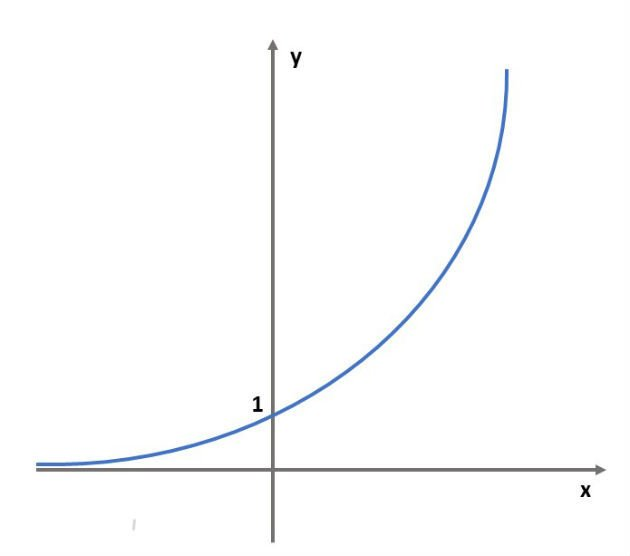
\includegraphics[width=0.7\linewidth]{expoencialgrafico1}
		\caption{Representação de uma função exponencial genérica.}
		\label{fig:expoencialgrafico1}
	\end{figure}
	Quando $ x $ é muito grande, a função "explode" e quando $ x $ é pequeno o suficiente ou um infinitesimal, a função se aproxima ao valor zero. Por sorte uma função exponencial cresce mais rápido do que qualquer polinômio e guardem essa informação quando forem trabalhar com limites, derivadas e integrais em um curso de cálculo.
	
	As funções exponenciais possuem algumas propriedades especiais e irei lista-las abaixo, seja $ a,b,m, n \in \mathbb{R} $, temos
	\begin{enumerate}
		\item $ a^ma^n=a^{m+n} $ \label{1}
		
		\item $ \frac{a^m}{a^n} = a^{m-n} $ \label{2}
		
		\item $ (ab)^n = a^nb^n $ \label{3}
		
		\item $ \left(\dfrac{a}{b}\right)^n = \dfrac{a^n}{b^n} $ \label{4}
		
		\item $ (a^m)^n = a^{mn} $ \label{5}
		
		\item $a^{\frac{m}{n}}= \sqrt[n]{m}$ \label{6}
	\end{enumerate}
	Essas propriedades são importantes para simplificar cálculos, escrever equações e termos convenientemente para algum resultado.
	
	Existe uma função exponencial especial que possui uma base que possui o valor $ e $ que também é chamado de número natural ou número de Euler, e por alguma razão decidida pela natureza, $ f(x) = e^x $ e funções parecidas/proporcionais aparecem bastante na descrição matemáticas de fenômenos físicos e problemas matemáticos.  Uma das formas de se calcular o número de Euler seria com a seguinte soma infinita
	
	\begin{equation}\nonumber
		\dfrac{1}{0!} + \dfrac{1}{1!} + \dfrac{1}{2!} +\dfrac{1}{3!}+ \dfrac{1}{4!}+\dfrac{1}{5!} + \cdots + \dfrac{1}{n!}= \sum_{n=0}^{\infty}\dfrac{1}{n!}.
	\end{equation}
	 Como eu já apresentei acima as definições e as propriedades de exponenciais, nada mais justo em resolver alguns exercícios passo a passo, mostrar como resolver as contas e depois propor exercícios para os leitores darem os próprios passos.
	 
	 \subsection{Exercícios resolvidos:}
	 Simplifique as expressões abaixo: 
	 \textbf{Se possível tente fazer os exercícios primeiro e depois leia a resolução.}
	 
	 \begin{enumerate}
	 	\item $ \dfrac{(a^5b^3)^4}{(a^2b^4)^2} $
	 	
	 	$$ \dfrac{(a^5b^3)^4}{(a^2b^4)^2} \text{  }= (\ref{3}) \Rightarrow \dfrac{(a^5)^4(b^3)^4}{(a^2)^2(b^4)^2}= (\ref{5}) \Rightarrow \dfrac{a^{20}b^{12}}{a^4b^8} = \dfrac{a^{16+4}b^{4+8}}{a^4b^8}= (\ref{1}) \Rightarrow \dfrac{(a^{16}b^4)(a^4b^8)}{a^4b^8} = a^{16}b^4$$
	 	
	 	\item $\dfrac{9}{2\sqrt{3}}$
	 	
	 	$$\dfrac{9}{2\sqrt{3}} = \left(\dfrac{1}{2}\right) \dfrac{9}{\sqrt{3}} = (\ref{6}) \Rightarrow \left(\dfrac{1}{2}\right) \dfrac{3^2}{3^{1/2}} = (\ref{2})  \left(\dfrac{1}{2}\right)3^{2-1/2} = \left(\dfrac{1}{2}\right)3^{3/2} = \dfrac{3^{3/2}}{2}$$
	 	
	 	\item $ \dfrac{a^{-1} + b^{-1}}{ab} $ onde $ (ab) \neq 0$
	 	
	 	$$ \dfrac{a^{-1} + b^{-1}}{ab} (\ref{2}) \Rightarrow = \dfrac{\frac{1}{a} + \frac{1}{b}}{ab} = \dfrac{\frac{a+b}{ab}}{ab}  = \dfrac{a+b}{(ab)^2}$$
	 	
	 \end{enumerate}
 
 	\subsection{Exercícios:}
 	Encontre o valor de x e utilize a prova real (substituindo o x) para verificar a sua resposta.
 	\begin{enumerate}
 		\item $ 9^x = 27 $
 		\item $ 16^{\frac{3}{x}} = \frac{1}{8}$
 		\item $ \pi^x = \frac{1}{\sqrt{\pi}} $
 		\item $ 9^{x^2+1} = 81 $
 		\item $ 2^{x^2 -4} = 128 $
 		\item $ 3^{x+2} + 3^x  = 2430 $
 		\item $ 3^{x^2-x} = 9 $
 		\item $ 5^{3x} = 64 $
 		\item $ 2^{x+3/2} = (1/2)^{-3} $
 		\item $ 2^{2x+1} \cdot 4^{3x+1} = 8^{x-1} $
 	\end{enumerate}
 	
	\section{Logaritmos}
	Os logaritmos são funções que possuem a seguinte forma
	\begin{equation}\nonumber
		f(x) = \log_a x,
	\end{equation}
	onde $ a $ é a base e $ x $ é o logaritmando e o seu resultado é o logaritmo.
	O logaritmo é a função inversa da função exponencial, ela cresce/diminui bem devagar em comparação com a exponencial, podemos ver o seu comportamento no gráfico abaixo.
	
	\begin{figure}[h!]
		\centering
		\includegraphics[width=0.45\linewidth]{../../Downloads/grafico-crescente-funcao-logaritmica-matematica}
		\caption{Representação do gráfico de uma função logarítmica genérica.}
		\label{fig:grafico-crescente-funcao-logaritmica-matematica}
	\end{figure}
	Quando a função logarítmica é aplicada em uma função é possível desvendar mudanças bruscas de comportamento de funções (quando as funções são tratadas como logaritmando).
	\newpage
	
	Como descrevi anteriormente, a função logarítmica é a inversa da função exponencial, uma definição formal seria dada por, seja a e b reais positivos diferentes de 1, o logaritmo de $ b $ na base $ a $ é o expoente $ x $ que satisfaz a igualdade $ a^x = b $. Em outras palavras,
	\begin{equation}
      \log_a b = x	\Leftrightarrow\ a^x = b.	\nonumber
	\end{equation}
	
	Assim como as exponenciais, os logaritmos possuem algumas propriedades especiais que são dadas por, seja $ a,b,c \in \mathbb{R}$ teremos
	\begin{enumerate}
		\item $\log_a 1 = 0$ \label{log1}
		
		\item $ \log_a a = 1 $ \label{log2}
		
		\item $ \log_a a^b = b \log_a \Rightarrow a = b $ \label{log3}
		
		\item $ a^{\log_a b} = b $ \label{log4}
		
		\item $\log_a b = \log_a c \Leftrightarrow b =0$ \label{log5}
		
		\item $ \log_a (b\cdot c) = \log_a b + \log_a c$ \label{log6}
		
		\item $  \log_a \frac{b}{c} = \log_a b - \log_a c $ com $ c \neq 0 $ \label{log7}
		
		\item $ \log_a b = \dfrac{\log_c b}{\log_c a} $ \label{log8}
		
		\item  $ \log_a b \log_b a = 1  $ \label{log9}
		
		\item $ \log_{a^c} b = \frac{\log_a b}{c} $ \label{log10}
	\end{enumerate}
		Essas propriedades são importantes para simplificar cálculos, escrever equações e termos convenientemente para estudar o comportamento de outras funções ao trata-la como logaritmando.
		
		Assim como nas exponenciais, existe uma logaritmo de especial relacionada ao número de Euler, o famoso "ln", isto é, $ \log_e \equiv \ln $ e esse logaritmo será visto muitas vezes em diversos cálculos, pois a natureza gosta bastante dele.
		
		Outro detalhe não menos importante, quando temos $ \log (x) $, significa que a base do logaritmo está omitida mas é convencionado que a base é 10.

		\subsection{Exercícios resolvidos:}
		Simplifique as expressões abaixo: 
		\textbf{Se possível tente fazer os exercícios primeiro e depois leia a resolução.}
		\begin{enumerate}
			\item $\log_6 12 - \log_6 3 $
			
			$$ \log_6 12 - \log_6 3 = \log_6 (3 \cdot 2) - \log_6 3 = (\ref{log6}) \Rightarrow  \log_63 - \log_62 - \log_6 3  = \log_62 $$
			
			\item $ 5^{-1 \log_52}$
			
			$$ 5^{-1 \log_52} = 5^{-1} \cdot5^{\log_52} = \ref{log4} \Rightarrow 5^{-1} 2 = \dfrac{2}{5}$$
	\end{enumerate}	

\subsection{Exercícios:}
Encontre o valor de x e utilize a prova real (substituindo o x) para verificar a sua resposta.
\begin{enumerate}
	\item $ \log_5 x = 0 $
	
	\item$  \log_2 (x+3) = 1  $
	
	\item $ \log_5 (x^2 -x ) = log_5 (8x-14) $
	
	\item  $\log_{27} x + \frac{1}{3}\log_3 2x =1  $
	
	\item  $ \log_3 x +\log_9 x = 1 $
	
	\item $ x = 16^{\log_45} $
	
	\item $\log_{10} (x+1) + \log_{x+3} = log_{10} 3$
	
	\item $ \dfrac{1}{\log_x8} + \dfrac{1}{\log_{2x} 8} + \dfrac{1}{\log_{4x} 8} = 2 $
	
	\item $ (\log_x 2)\cdot(\log_{\frac{x}{16}} 2) = \log_{\frac{x}{64} 2} $
	
	\item $ \log_{\pi} (\pi x^2) - 1 = -\log_{\pi^2} \left(\dfrac{1}{\pi^4}\right) $
\end{enumerate}
			
			
\textbf{Aproveitem o material queridos!}

\begin{figure}[h!]
	\centering
	
\includegraphics[width=0.25\linewidth]{istockphoto-481013807-170667a}
	\caption{Descoberta do $\ln 0$.}
	\label{fig:istockphoto-481013807-170667a}
\end{figure}

			
			
			
			
			
			
			
			
			
			
			
			
			
			
			
			
			
			
			
			
			
			
			
		
		
		
		
\end{document}